%!TEX root = ../../../2019main.tex

\vspace{10pt}
\subsubsection*{\bf Commissioning}
\vspace{3pt}
\noindent {\sf [Spokesperson :\ Osamu MIYAKAWA]}

\vspace{3pt}
\noindent {\sf \small ICRR, The Univ.\ of Tokyo, Hida, Gifu 506-1205}

\vspace{3pt}

For KAGRA, it is not an exaggeration to say that the fiscal year of 2019 has been a year of commissioning. By FY2018, almost all of the subsystems had been installed and in FY2019 we targeted to operate as a whole interferometer. We had several engineering runs with the Michelson interferometer, operating in a single arm cavity, and finally carried it through to observation. It is a remarkable result that we were able to achieve the minimum target sensitivity of 1 MPc. This led to a joint observation with GEO.

In this process, one major problem was exposed: the presence of birefringence in the Sapphire mirror, which was thought to reduce the returning light from the interferometer.  This can be a direct problem for sensitivity since the target power-recycling gain cannot be achieved. It was then found that the modal healing effect of the arm cavity relieved this problem and that sufficient power recycling gain could be obtained. However, the sidebands would still be lost due to the birefringence, so we should consider making the mirror again in order to achieve the final sensitivity.

\begin{figure*}[htbp]
\begin{center}
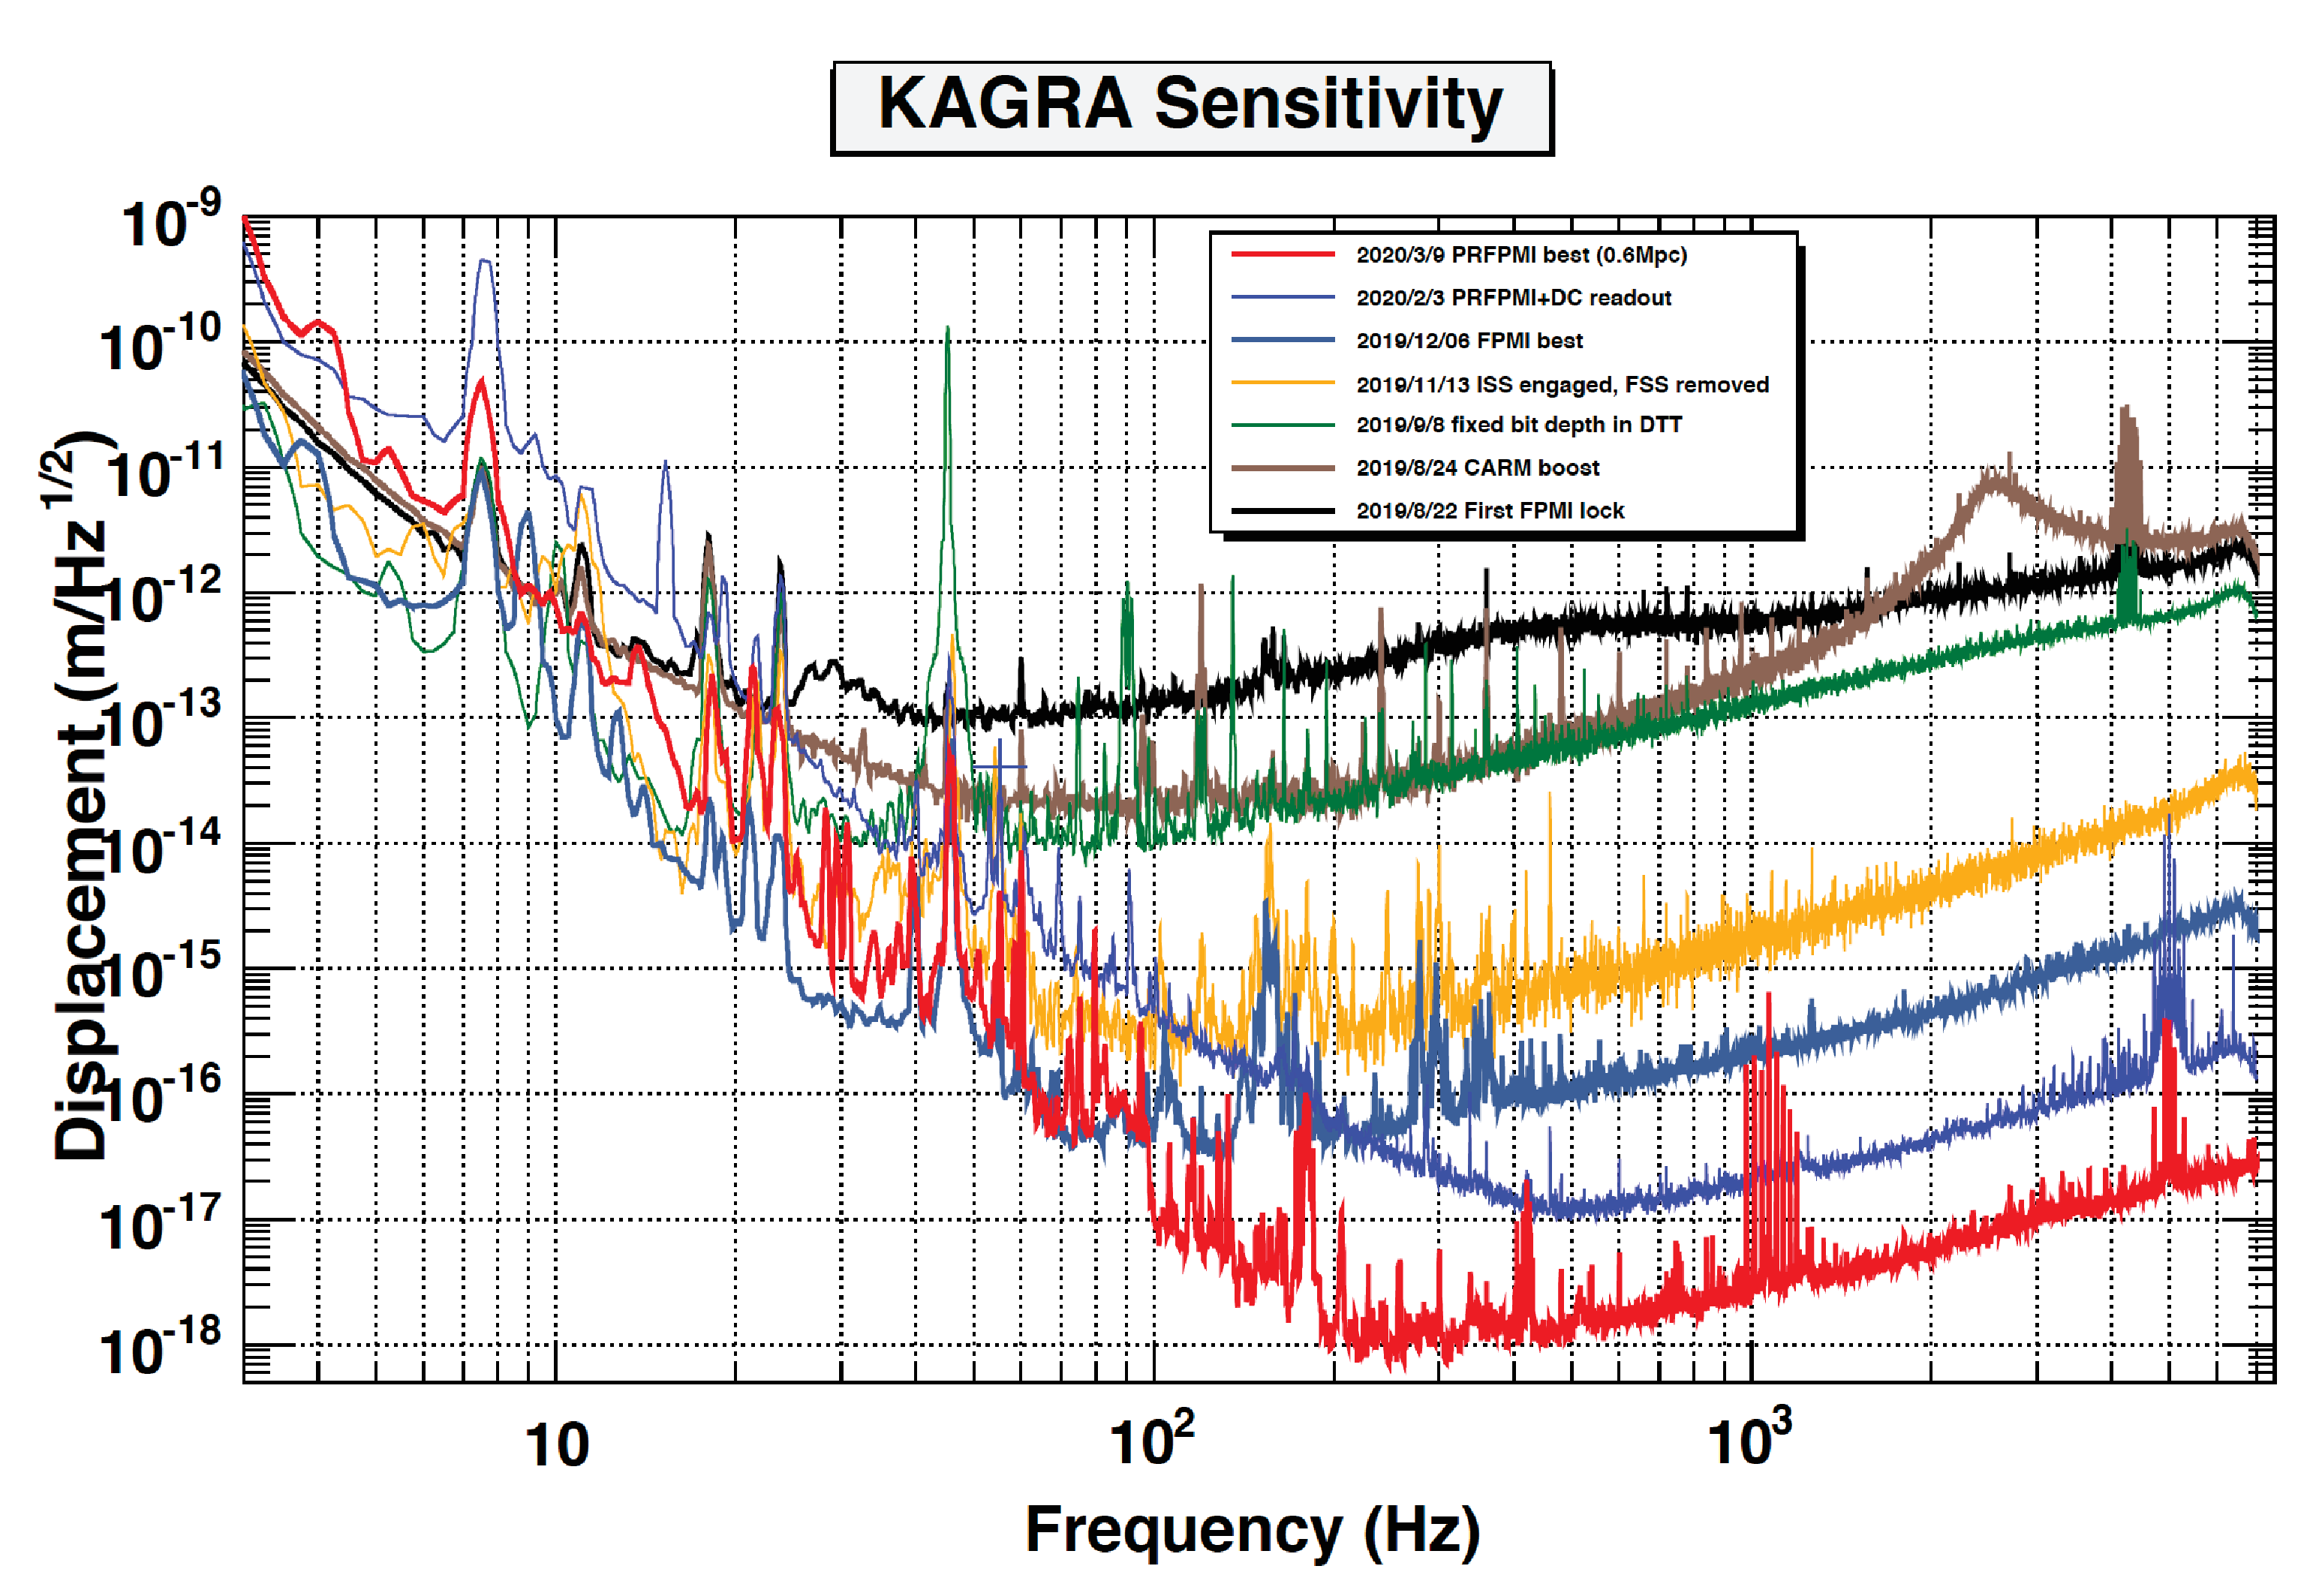
\includegraphics[width=14cm]{astrodiv/gw/commissioning/sens_improve.eps}
\caption{Improvement of the KAGRA sensitivity in 6 months.}
\label{fig:sens_improve}
\end{center}
\end{figure*}


The Fig.\ref{fig:sens_improve} shows the improvement in sensitivity over a period of about six months. We successfully achieved the first FPMI operation in late August, with both 3\,km arms  storing light into the arm cavities, and the first sensitivity was measured. At this point, it was found that 4-5 orders of magnitude were necessary to reach the minimum target sensitivity, and we realized that noise-hunting was the most important task for commissioning. We improved the sensitivity initially by resolving a few minor problems. When the sensitivity improvement was a bit slow, the introduction of the ISS (Intensity Stabilization Servo) improved by one order, and the removal of the FSS (Frequency Stabilization Servo) improved by another order of magnitude, total improvement in sensitivity by two orders of magnitude was not insignificant at that time. We continued to try to improve the sensitivity, but since we were using only 10\% of the transmitted light of the power recycling mirror, it was difficult to increase the laser power in the interferometer further, which limited the sensitivity at high frequencies.

In January, the PRFPMI which aimed to increase laser power in the interferometer was successfully operated. The laser power could be increased by a factor of 100 compared to the FPMI state. Although there were some concerns about the noise in the control systems, it was found that they did not limit the final sensitivity of the PRFPMI for the observations in 2019, and the operation of PRFPMI was fine. However, we believe that we need to move to DRFPMI to realize the final sensitivity as designed.

The following February we successfully established the OMC (output mode cleaner) in operation. This OMC allowed us to measure the sensitivity of the interferometer using DC power. This is called as a DC readout method that was designed as an final method without using RF sideband signals. The first sensitivity of the DC readout was 40\,kpc, which was almost the same as the highest sensitivity of FPMI, and we aimed to improve the sensitivity further. From this point, we improved the sensitivity by one more order of magnitude, and when the sensitivity was about 400\,kpc, we started the first observation for two weeks. During the observation, the sensitivity fluctuated several times due to uncertainties of calibration. This issue is still under investigation, and further verification is necessary. Finally, we achieved the minimum target sensitivity of 1\,Mpc, and this led to the second round of observations in April.

Through this commissioning, it was found that both sensitivity and stability are highly dependent on the alignment of mirrors. The angular control of the mirror has been successfully introduced in some degrees of freedom. In order to achieve the final sensitivity, it is necessary to introduce the angular control for all the degrees of freedom. It was also exposed that weakness for climate change, such as micro seismic motion in the 0.1 Hz band existed. This needs to be resolved by improving the control system of the vibration isolation system.

There were various problems and issues during the commissioning process, and most of them were solved and the stable operation was achieved. Although, there are still some problems to be solved, but it is remarkable that we have established the 4-5 orders of magnitude improvement of the sensitivity in only 6\,months. In the future, we will update the vibration isolation system and try to achieve the final target sensitivity through further commissioning.



